\documentclass[a4paper, 11pt]{article}
\usepackage[margin=1in]{geometry}
\usepackage{amsmath}
\usepackage{graphicx}
\usepackage{tikz}
\usepackage[hidelinks]{hyperref}
\usepackage{color}
\usepackage{xcolor}
\usepackage{listings}
\usepackage{float}

\lstset{basicstyle=\small}

\usepackage{caption}
\DeclareCaptionFont{white}{\color{white}}
\DeclareCaptionFormat{listing}{\colorbox{gray}{\parbox{\textwidth}{#1#2#3}}}
\captionsetup[lstlisting]{format=listing,labelfont=white,textfont=white}

\begin{document}
%Header-Make sure you update this information!!!!
\noindent
\large\textbf{Obligatory Assignment 1 Report} \hfill \textbf{Tomasz Gliniecki} \\

\section*{Problem Statement}
\subsection*{Monty Hall problem}
The most effective strategy \emph{in the long run} is to ALWAYS SWITCH. This is because, one has always $\frac{2}{3}$ chance of winning by swithcing. This is obvoius because, there is $\frac{1}{3}$ chance of finding the prize which is behind 1 of the 3 gates, that means that there is $\frac{2}{3}$ chance of NOT finding the prize. If we set our goal to NOT find the prize, and then switch when the empty gate opens, we will win with a $\frac{2}{3}$ probability, because there is $\frac{2}{3}$ chance of not finding the prize!\\
The simulation from [Listing\ref{lst:keepmonty}] shows that there is approximately $ ~[1] 0.6771 $ chance of winning with strategy 2. So the recommended strategy is strategy 2, always switch.

\subsection*{Rock Paper Scissors}
There is $\frac{1}{3}$ chance of choosing either of the shapes. Probability for a person to NOT choose any given shape is $\frac{2}{3}$ because then it leaves out 2 other possibilities of 3. Whatever the person chooses has no influence on what the other chooses, that means there is $\frac{2}{3}$ chance for one person to choose something else than the first person, thus giving $\frac{2}{3}$ chance for the game to end successfully, game ends in succes if the choices differ. The possible outcomes are success (someone winning) with 2/3 probability, and failure (a tie) 1/3 probability, since the trails are independant, the probability of succes is the same on each trial this tells us that geometrical distribution is an appropriate model.\\
The expected number of trials until there is a winner is:
\begin{center}$ 1/\frac{2}{3}  $\end{center}\
The results of k = 1 from the simulation is very close to
\begin{center}$ 1/\frac{2}{3} =1.5 $\\$1.503$\end{center}

The probability $ P(X \leq 5) $, X being five or less, is
\begin{center}$ P(X=5) + P(X=4) + P(X=3) + P(X=2) + P(X=1)  $\end{center}
\begin{center}$ P(X=x)=(1-p)^{x}\,p\,  $\end{center}
\begin{center}$ P(X\leq5) = \sum_{i=0}^{5} (1-\frac{2}{3})^{i}\,\frac{2}{3} = 0.996$\end{center}

The R function that returns the number of trials is shown in [Listing\ref{lst:ntrials}]. Results of checking the routine for k = 1 gives us either 2 or 1 as the return value, which is what we would expect. Simulating it $10^5$ times gives us approximations that are show below in histogram for k=1s [Figure \ref{k1}].
\begin{figure}[H]
  \centering
  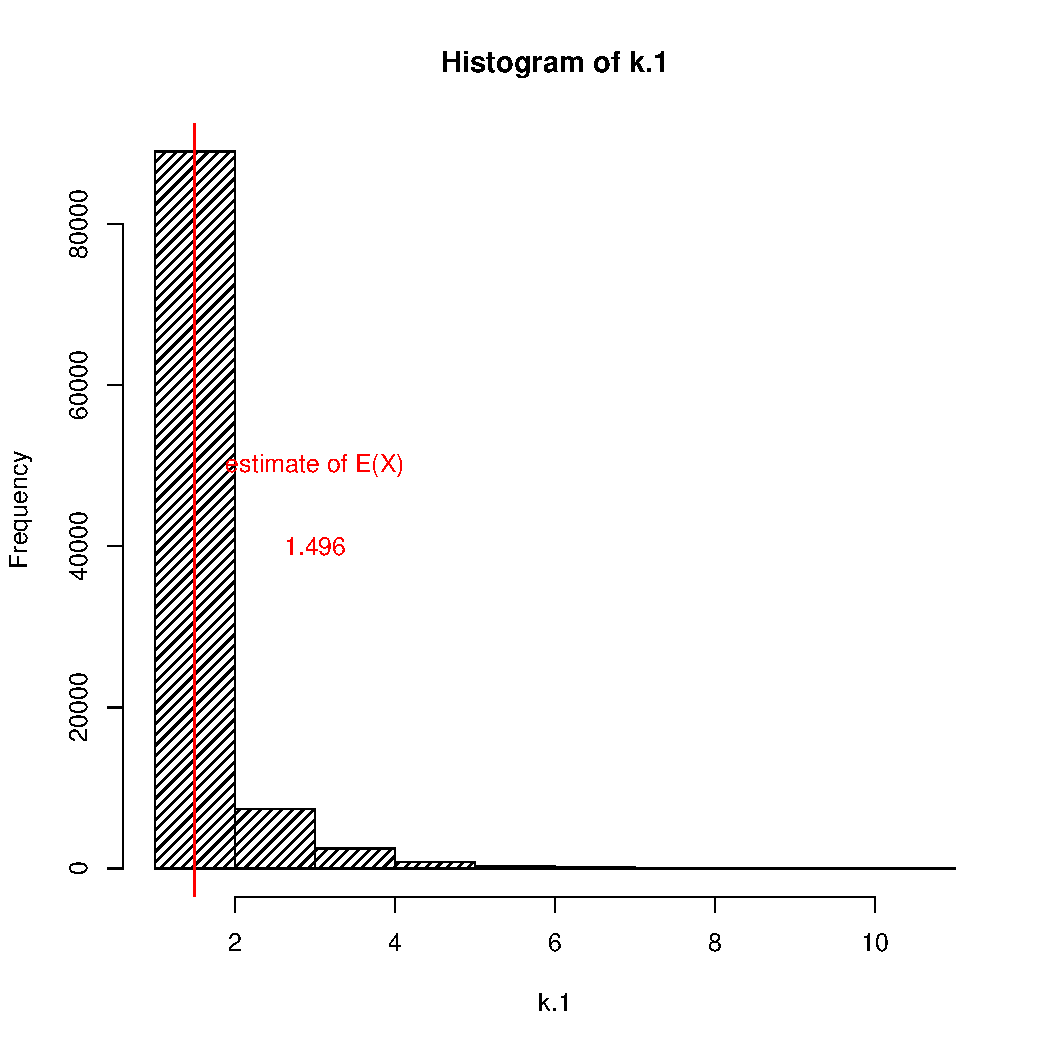
\includegraphics[scale=0.7,page=1]{Rplots.pdf}
  \caption{Simulation of k = 1}
  \label{k1}
\end{figure}


The estimated number of trials untill there is a winner for k=3 and k=5 after $10^5$ simulations is as follows:
\\\\
Probability $ P_{k=3}(X\leq8) $ and $ P_{k=5}(X\leq8) $
\\\\
for $k=3$ $ P(X\geq8) = 0.237 $ see fig.\ref{k3}
\\
for $k=5$ $ P(X\geq8) = 0.907 $ see fig.\ref{k5}


\begin{figure}[H]
  \centering
  \includegraphics[scale=0.7,page=2]{Rplots.pdf}
  \caption{Simulation of 3 lives}
  \label{k3}
\end{figure}

\begin{figure}[H]
  \centering
  \includegraphics[scale=0.7,page=3]{Rplots.pdf}
  \caption{Simulation of 5 lives}
  \label{k5}
\end{figure}

\newpage
\section*{Construction/Implementation}
\begin{lstlisting}[caption={Simulation of "swtich" strategy in Monty Hall problem},label={lst:keepmonty},language=C++]
for (i in c(0:1e4)) {
  gate_distribution <- sample(possible_items, prob=c(1/3,1/3,1/3));
  contestant_choice <- sample(possible_choices,size=1,prob=c(1/3,1/3,1/3));
  # amount of wins strategy 2
  if ("car" %in% gate_distribution[-contestant_choice]) {
  switch <- switch+1;
  }
}
\end{lstlisting}

\begin{lstlisting}[caption={Number of trials needed to finish the game given k lives},label={lst:ntrials},language=C++]
play_rps <- function(lives=1) {
  k <- 0;
  while(1) {

    #independent choices
    player0 <- sample(elements,size=1,prob=p);
    player1 <- sample(elements,size=1,prob=p);

    ifelse ((player0==''R'' && player1==''S''), p0win <- p0win+1,
    ifelse ((player0==''R'' && player1==''P''), p1win <- p1win+1,

    ifelse ((player0==''P'' && player1==''R''), p0win <- p0win+1,
    ifelse ((player0==''P'' && player1==''S''), p1win <- p1win+1,

    ifelse ((player0==''S'' && player1==''P''), p0win <- p0win+1,
    ifelse ((player0==''S'' && player1==''R''), p1win <- p1win+1,NA))))));

    k <- k+1;

    if (p0win>=lives || p1win>=lives) {
      break
    }
  }

  return(k);
}
\end{lstlisting}

\section*{Attachments}

montyhallproblem.R rps.R Rplots.pdf

\begin{thebibliography}{9}
  
\bibitem{montyhall} 
  Monty Hall problem, [cited 27.September 2016]. Available at \url{https://en.wikipedia.org/wiki/Monty_Hall_problem}

\end{thebibliography}

\end{document}
